% !TeX root = ../main.tex
% !TEX root = ../main.tex
% -*- root: ../main.tex -*-
% -*- program: pdflatex -*-
\chapter{构造公式方法}
上一章主要从插值方法入手介绍了对TOF的MRPC的离线数据的刻度方法。这一章将从构造公式入手对此刻度进行研究。仍然采用~Z~和~TOT~分开修正的方法。其中对于~Z~的修正采用简单的多项式构造,对于~TOT~的修正,通过分析时间对~TOT~的分布,构造出几种简单的公式,并比较拟合的情况和拟合的结果,最终确定~TOT~项的公式。

\begin{figure}[!h]
\begin{minipage}[!h]{0.5\linewidth}
%\centering
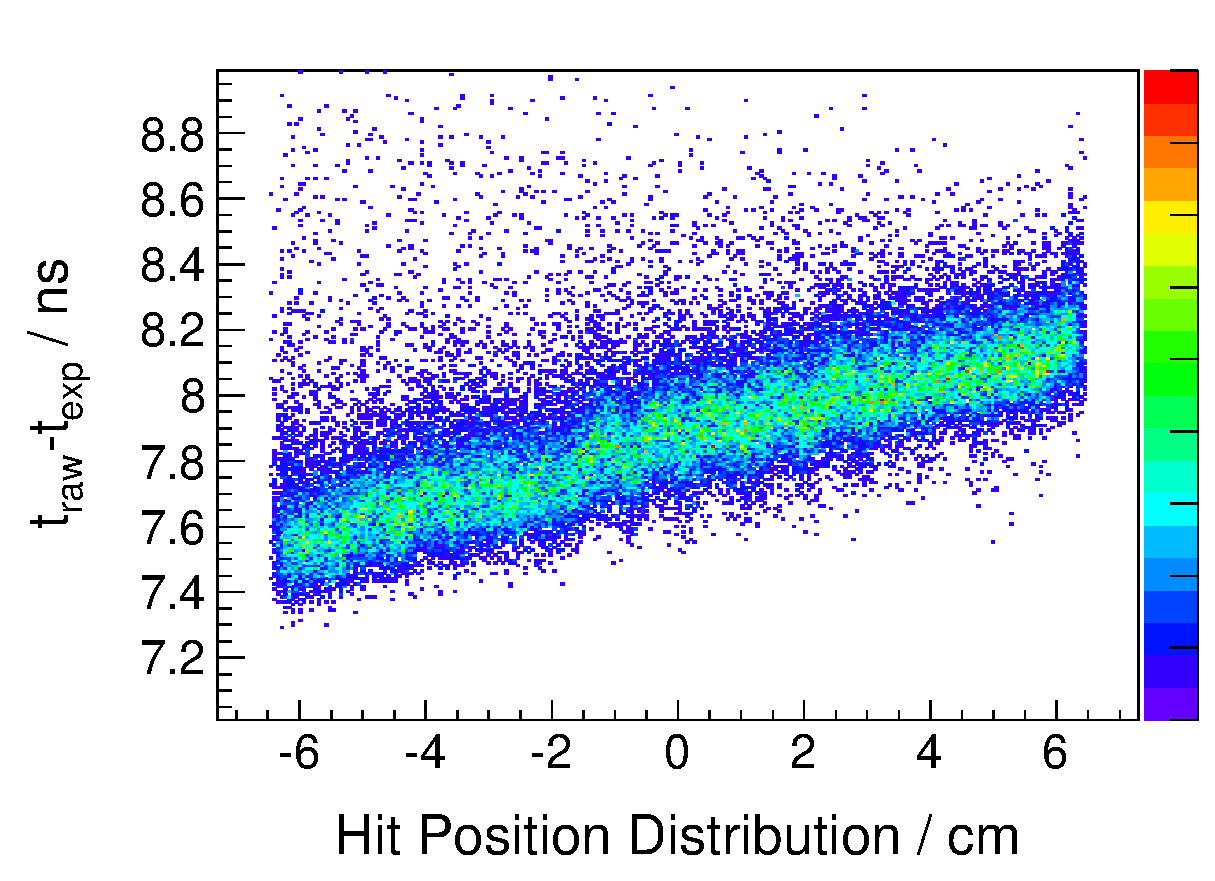
\includegraphics[width=0.9\textwidth]{chap3/left-tVSz.eps}
\subcaption{时间对~Z~的分布}
\label{fig:left-tVSz}
\end{minipage}%
\hfill
\begin{minipage}[!h]{0.5\linewidth}
%\centering
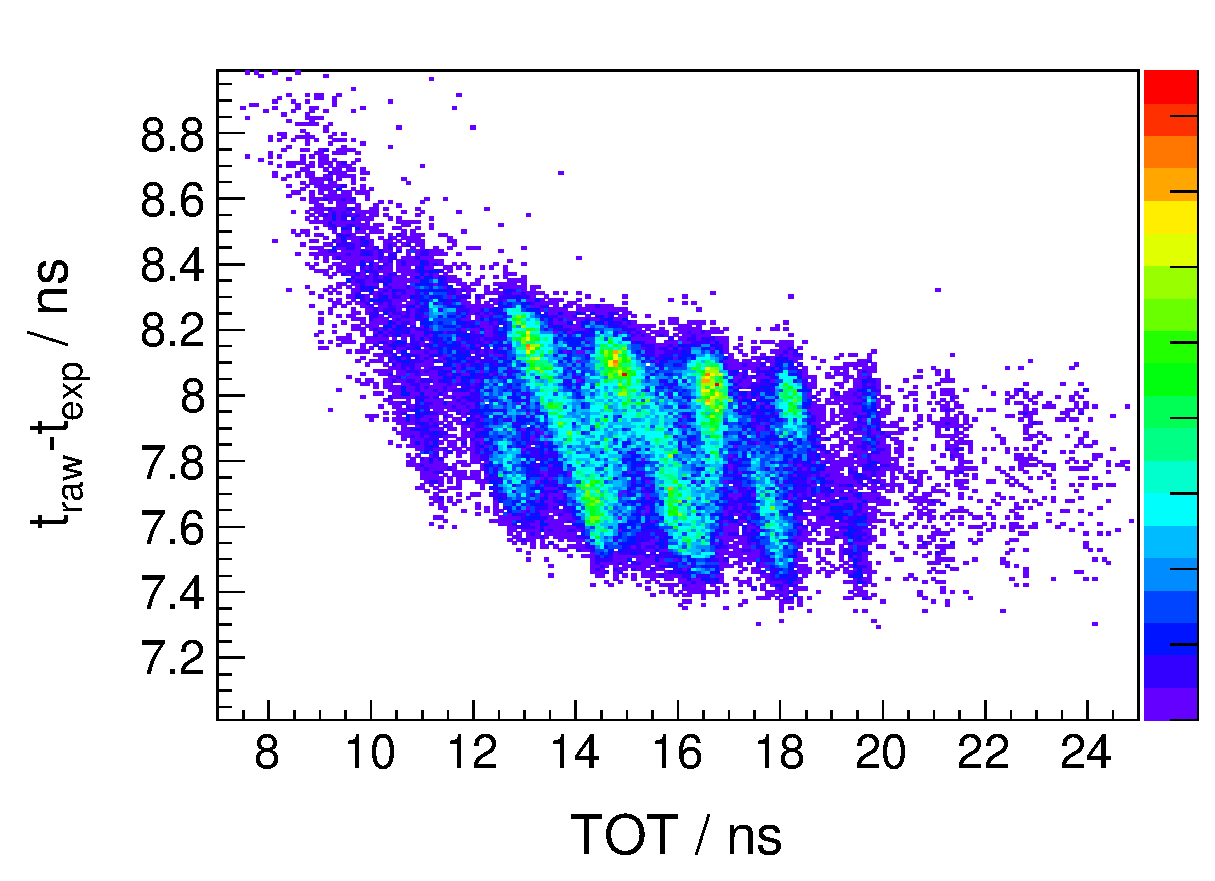
\includegraphics[width=0.9\textwidth]{chap3/left-tVSq.eps}
\subcaption{时间对~TOT~的分布}
\label{fig:left-tVSq}
\end{minipage}
\caption{时间对~Z~和~TOT~的分布}
\end{figure}

\section{~Z~的修正}
刻度修正的主要项之一就是~Z~项的修正。图~\ref{fig:left-tVSz}~时间与~Z~项的分布关系相对简单,几乎是线性关系。这一项主要是信号在对数条内的传播时间。
\subsection{Z~向等区间分~bin~}

\begin{figure}[htbp]
\centering
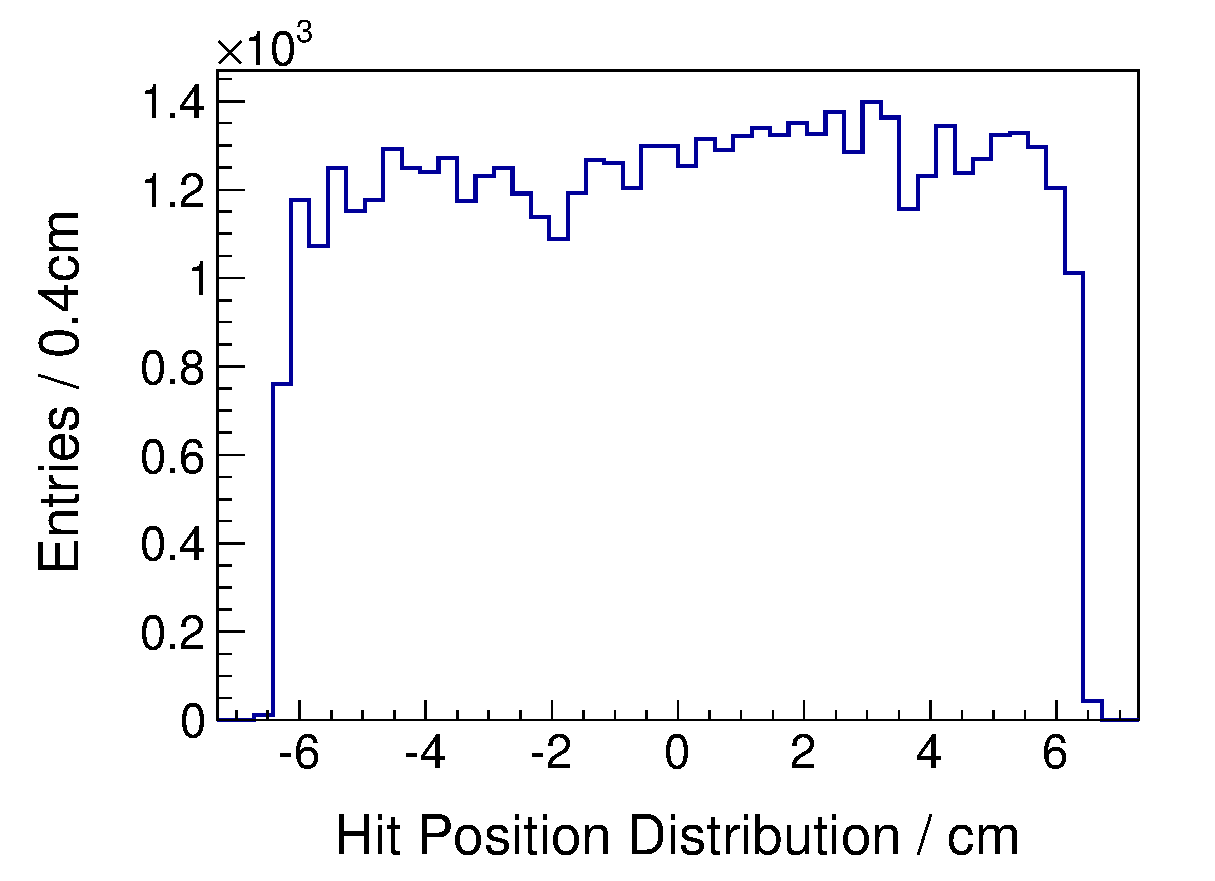
\includegraphics[width=0.5\textwidth]{chap3/left-z.eps}
\caption{~Z~的分布}
\label{fig:left-z}
\end{figure}

图~\ref{fig:left-z}~是击中位置~Z~的分布。可以看出,在此方向上事例数是均匀分布的,因此对~Z~的分~bin~采用等区间分~bin~。

图~\ref{fig:13bin}~是单个~bin~的时间分布。可以看出,这个分布左右并不完全对称,故不适合采用高斯拟合。考虑过采用朗道卷积一个高斯的拟合,但拟合的也并不十分贴切。

\begin{figure}[htbp]
\centering
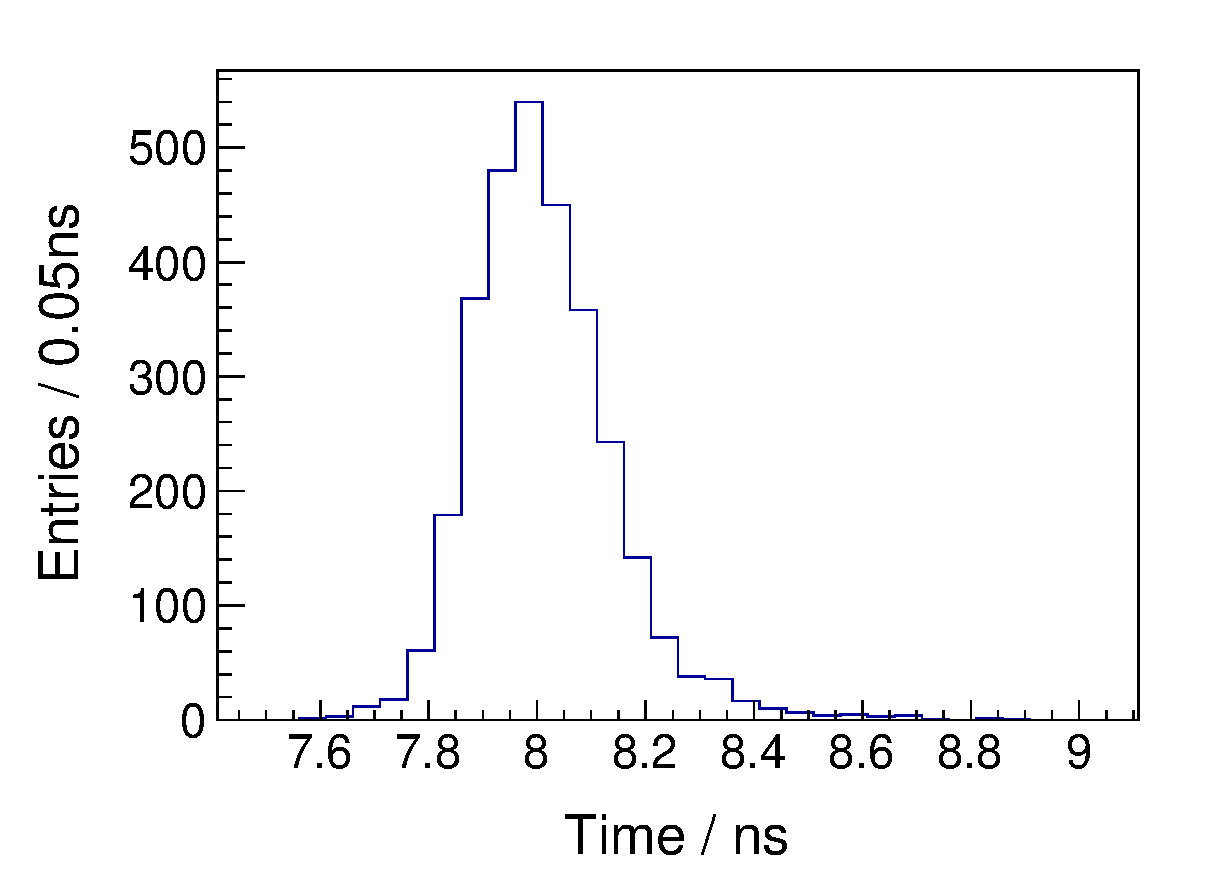
\includegraphics[width=0.5\textwidth]{chap3/13bin.eps}
\caption{单个~bin~的时间分布}
\label{fig:13bin}
\end{figure}

\subsection{每个~bin~采用~Nov~公式拟合}

从之前边渐鸣文章~Abosolute photon energy calibration for the BESIII EMC~ \cite{Bian:2010aa}~中看到关于${e^{+}e^{-} \to \gamma \gamma}$的分布也是左右不对称的,拟合采用的是一个~Novosibirsk~的公式。
关于这个公式:
\begin{displaymath}
f_{Nov}(m)=Aexp(\frac{-ln^2(1+t\frac{sinh(t\sqrt{ln4})}{t\sqrt{ln4}}\frac{m-m_{0}}{\sigma})}{2t^2}-\frac{t^2}{2}) %~\cite{Nov:2000aa}~
\end{displaymath}


~A~表示归一化常数,~$\sigma$~
表示时间分辨,~$m_{0}$~表示中心值,~$t(<0)$~表示参数化的尾巴。这个函数可以被看做是有一个不对称的尾巴的高斯函数。分析发现,这个函数形式对于拟合图~\ref{fig:13bin}~很合适。

\begin{figure}[htbp]
\centering
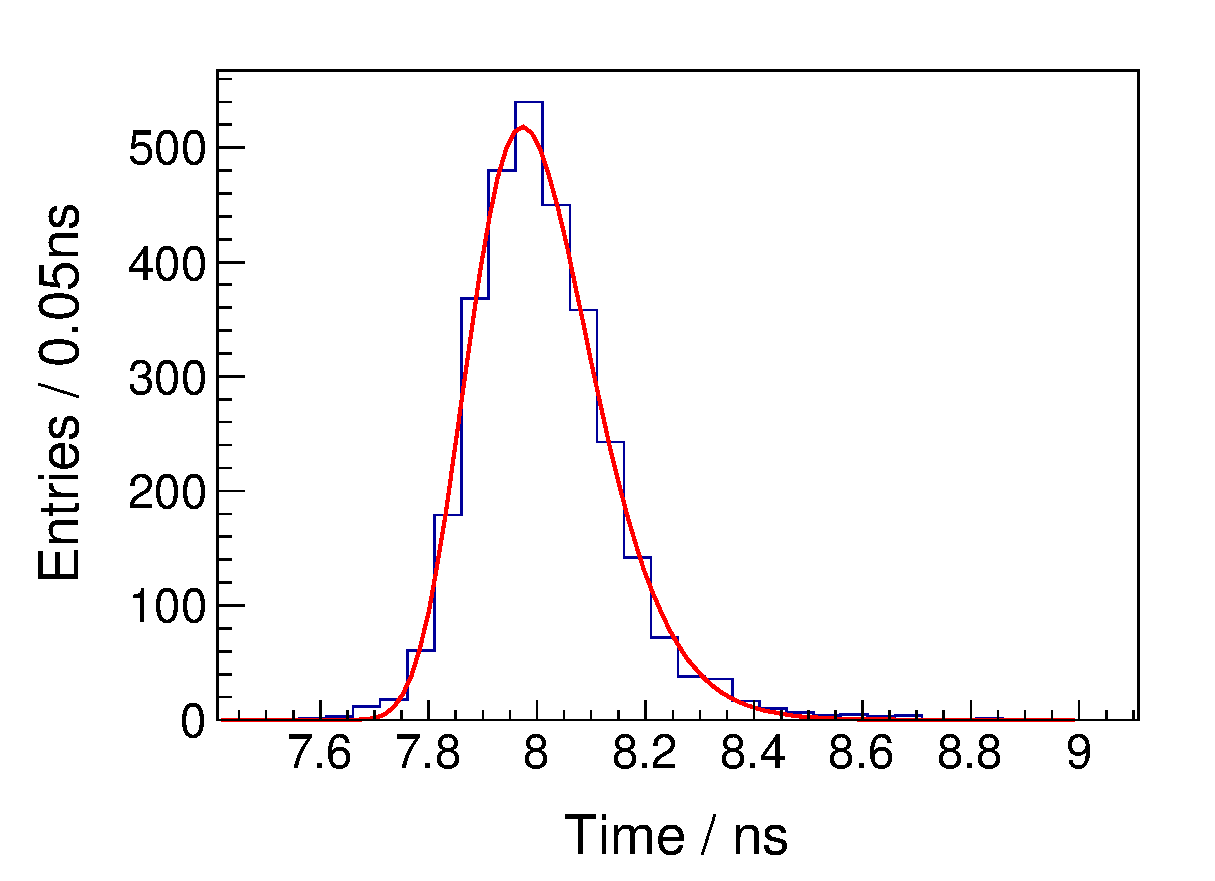
\includegraphics[width=0.5\textwidth]{chap3/13BinDraw.eps}
\caption{单个~bin~的时间用~Nov~公式拟合的结果}
\label{fig:13BinDraw}
\end{figure}

图~\ref{fig:13BinDraw}~是单个~bin~采用Nov公式拟合的结果。可以看出拟合的很好。

\begin{figure}[htbp]
\centering
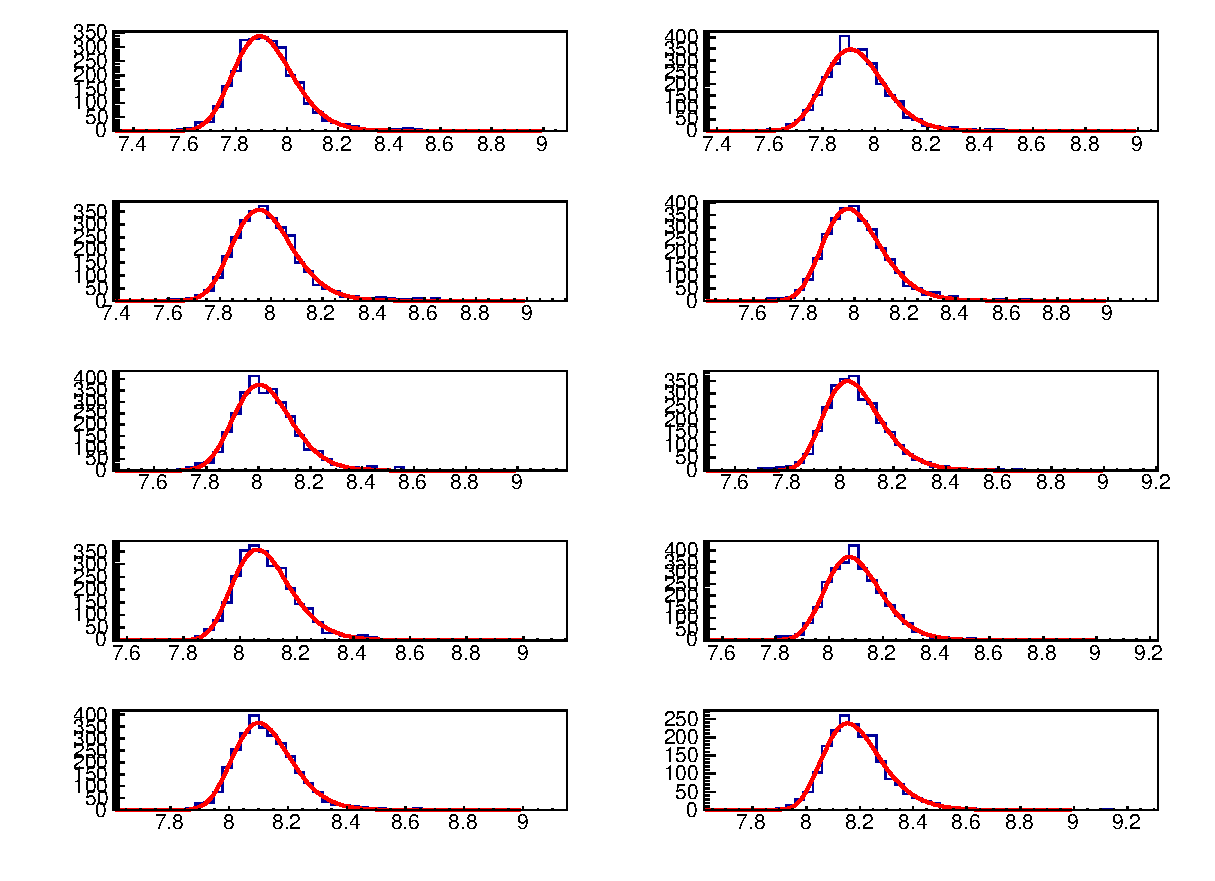
\includegraphics[width=0.6\textwidth]{chap3/10geDraw.eps}
\caption{10个~bin~的时间用~Nov~公式拟合的结果}
\label{fig:10geDraw}
\end{figure}

然后尝试~Nov~公式对10个~bin~拟合情况。见图~\ref{fig:10geDraw}~,可以看出每个~bin~的拟合都比较好。所以对于~Z~分~bin~后就采用~Novsibirsk~公式进行拟合。

\subsection{对得到的~graph~点采用三阶多项式拟合}
上一小节研究得到了分~bin~后的每个~bin~的中心值。对此采用一个多项式拟合。如图~\ref{fig:z-fit}~

\begin{figure}[htbp]
\centering
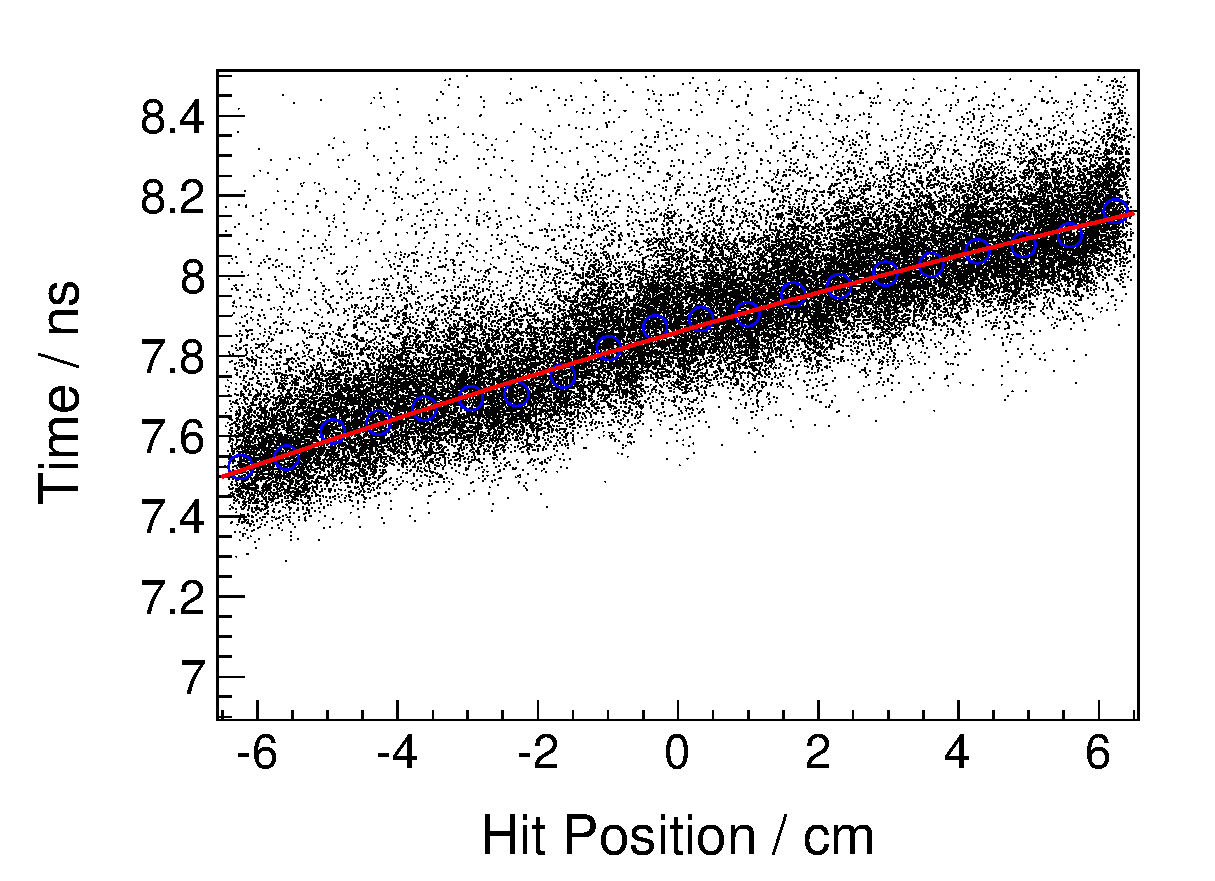
\includegraphics[width=0.8\textwidth]{chap3/z-fit.eps}
\caption{对~Z~三阶多项式拟合}
\label{fig:z-fit}
\end{figure}

选用三阶多项式的原因,是因为更低阶的多项式不能完全拟合出时间对~Z~的趋势,而更高阶的多项式也不能拟合的更出色了。

\section{TOT~的修正}

图~\ref{fig:afterCorZ-TOT}~是利用上述方法修正完~Z~后的时间对~TOT~的分布,此时时间对~TOT~的分布已经比修正~Z~前的时间和~TOT~的分布简单了。

\begin{figure}[htbp]
\centering
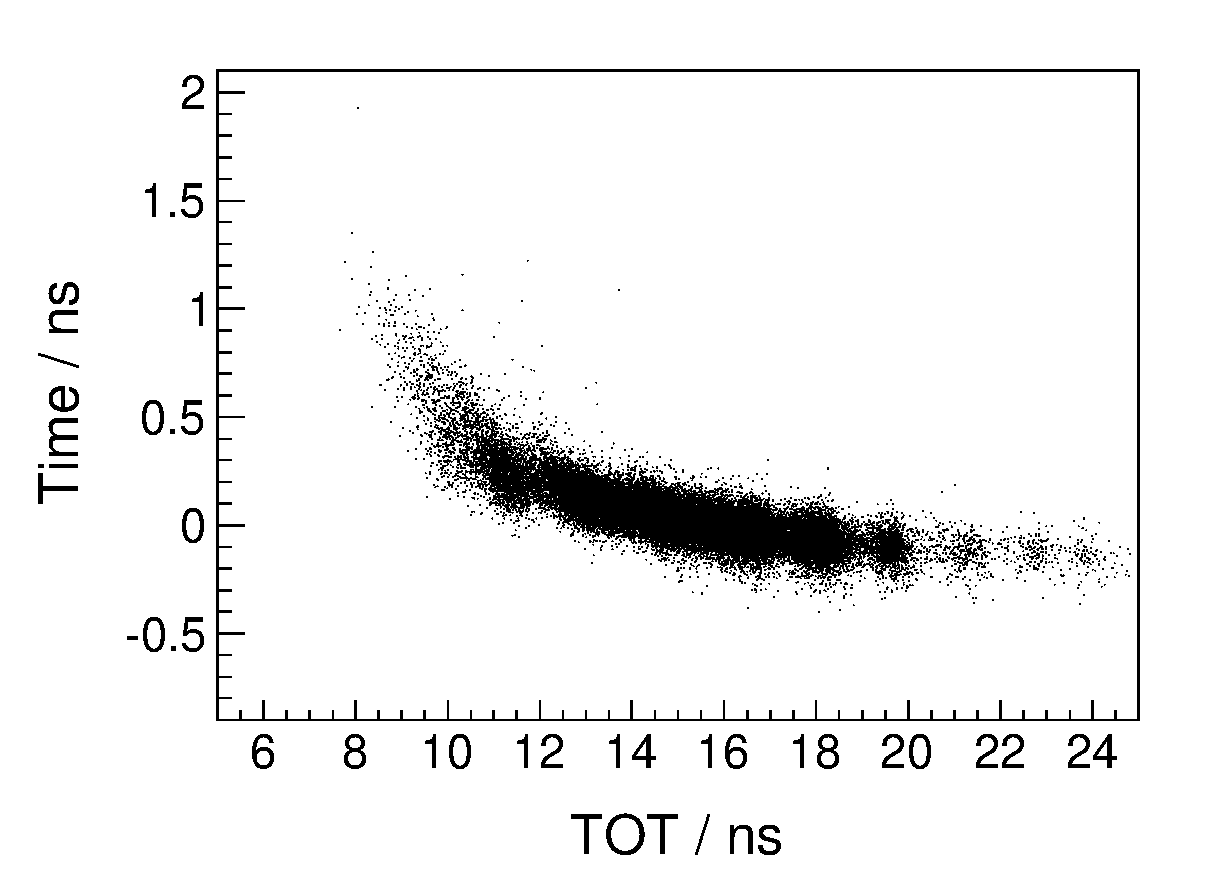
\includegraphics[width=0.8\textwidth]{chap3/afterCorZ-TOT.eps}
\caption{~Z~修正后时间对~TOT~的分布}
\label{fig:afterCorZ-TOT}
\end{figure}

基于此种分布,选用以下几种公式进行尝试,分别是:

\begin{align}
p_{0}+p_{1}/\sqrt{q}
\label{eq:1}\\
p_{0}+p_{1}/q
\label{eq:2}\\
p_{0}+p_{1}/q^{2}
\label{eq:3}\\
p_{0}+p_{1}/q^{3}
\label{eq:4}\\
p_{0}+p_{1}/\sqrt{q}+p_{2}/q
\label{eq:5}\\
p_{0}+p_{1}*q+p_{2}*q^{2}+p_{3}*q^3
\label{eq:6}    
\end{align}

比较公式~\ref{eq:1}~,~\ref{eq:2}~,~\ref{eq:3}~,~\ref{eq:4}~,~\ref{eq:5}~,~\ref{eq:6}~拟合的好坏,以及最终的时间分辨,分辨随~Z~和~TOT~,~tofid~,~strip~等的分布,决定哪个是时间与~TOT~关系的主项。

\subsection{尝试各种公式}

\begin{figure}[h]
\begin{minipage}{0.5\linewidth}
  \centerline{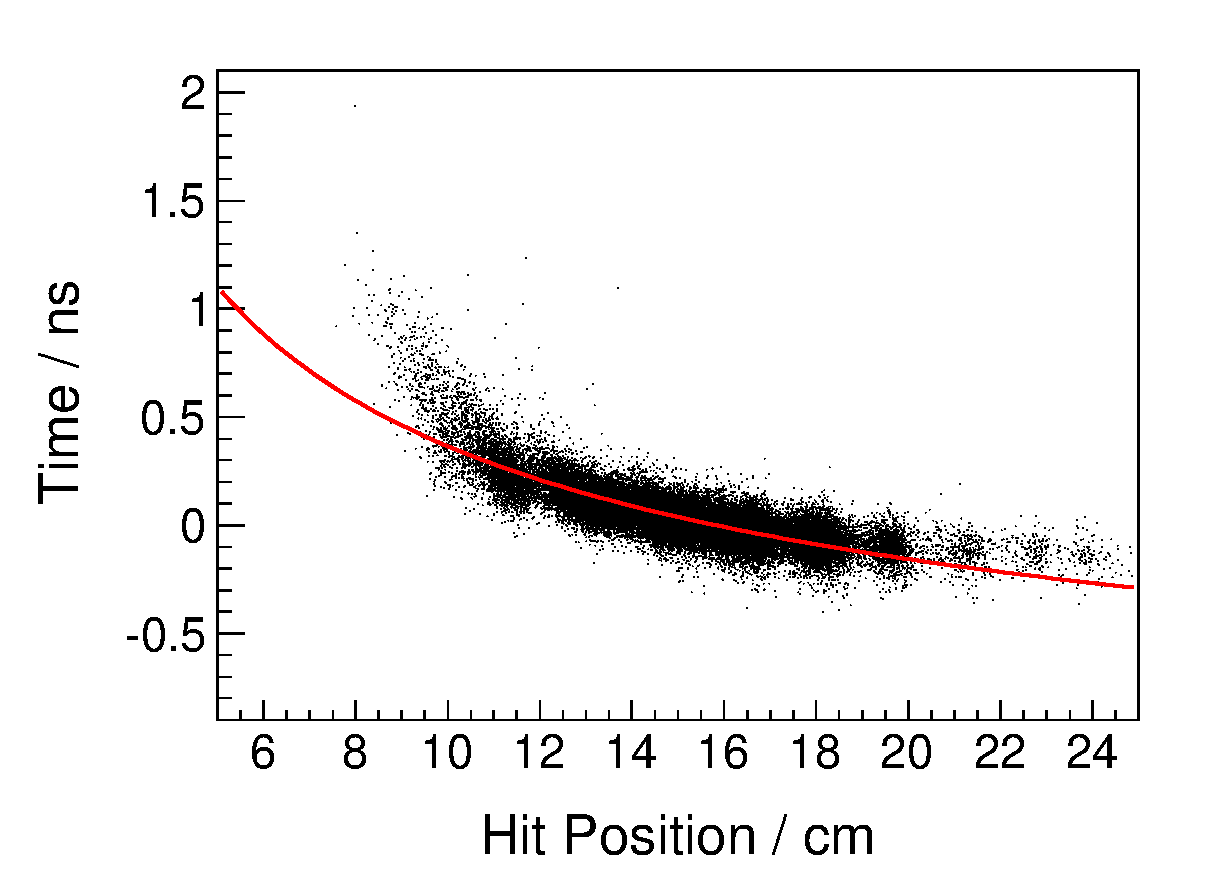
\includegraphics[width=0.9\textwidth]{chap3/ban-order.eps}}
  \centerline{(a) 公式~\ref{eq:1}~的拟合}
  \centerline{\label{fig:ban-order}}
\end{minipage}
\hfill
\begin{minipage}{0.5\linewidth}
  \centerline{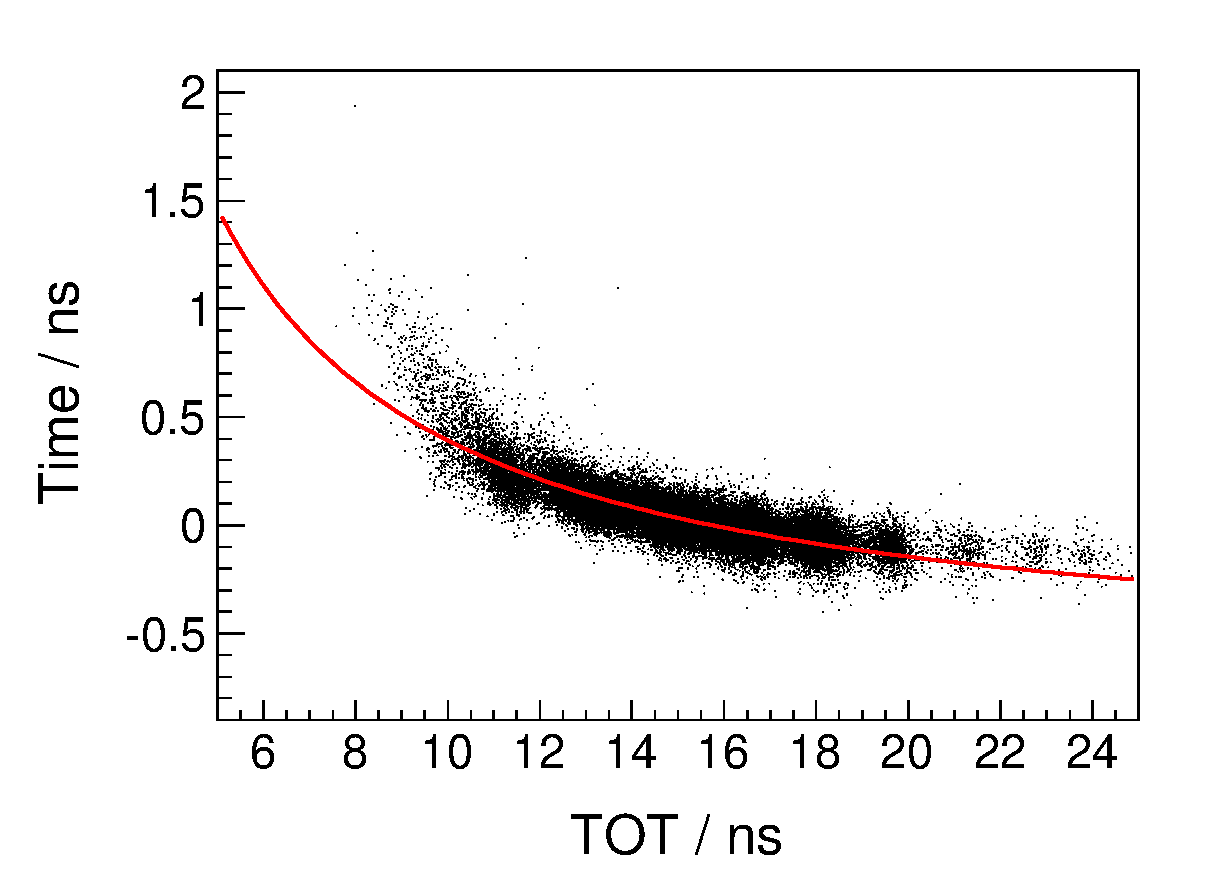
\includegraphics[width=0.9\textwidth]{chap3/1-order.eps}}
  \centerline{(b) 公式~\ref{eq:2}~的拟合}
  \centerline{\label{fig:1-order}}
\end{minipage}
\vfill
\begin{minipage}{0.5\linewidth}
  \centerline{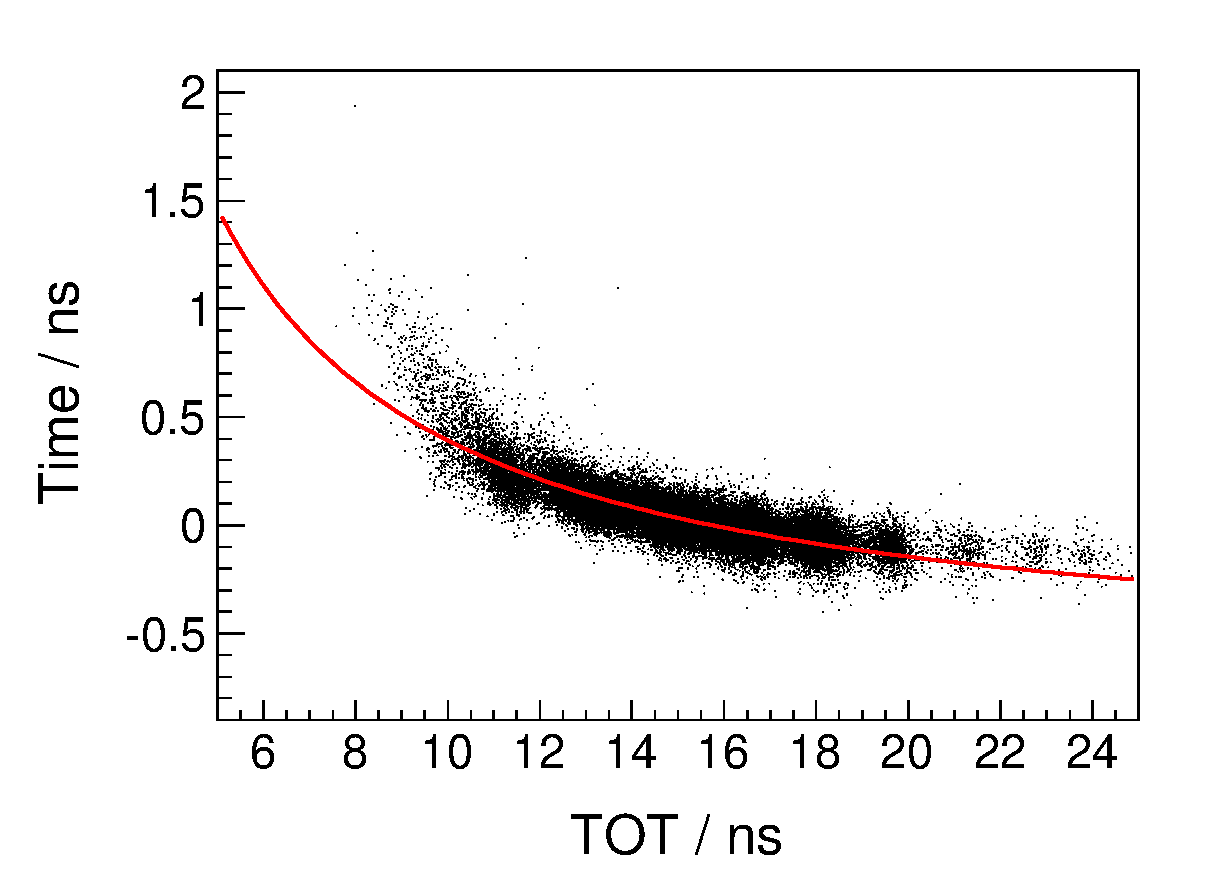
\includegraphics[width=0.9\textwidth]{chap3/1-order.eps}}
  \centerline{(c) 公式~\ref{eq:3}~的拟合}
  \centerline{\label{fig:2-order}}
\end{minipage}
\hfill
\begin{minipage}{0.5\linewidth}
  \centerline{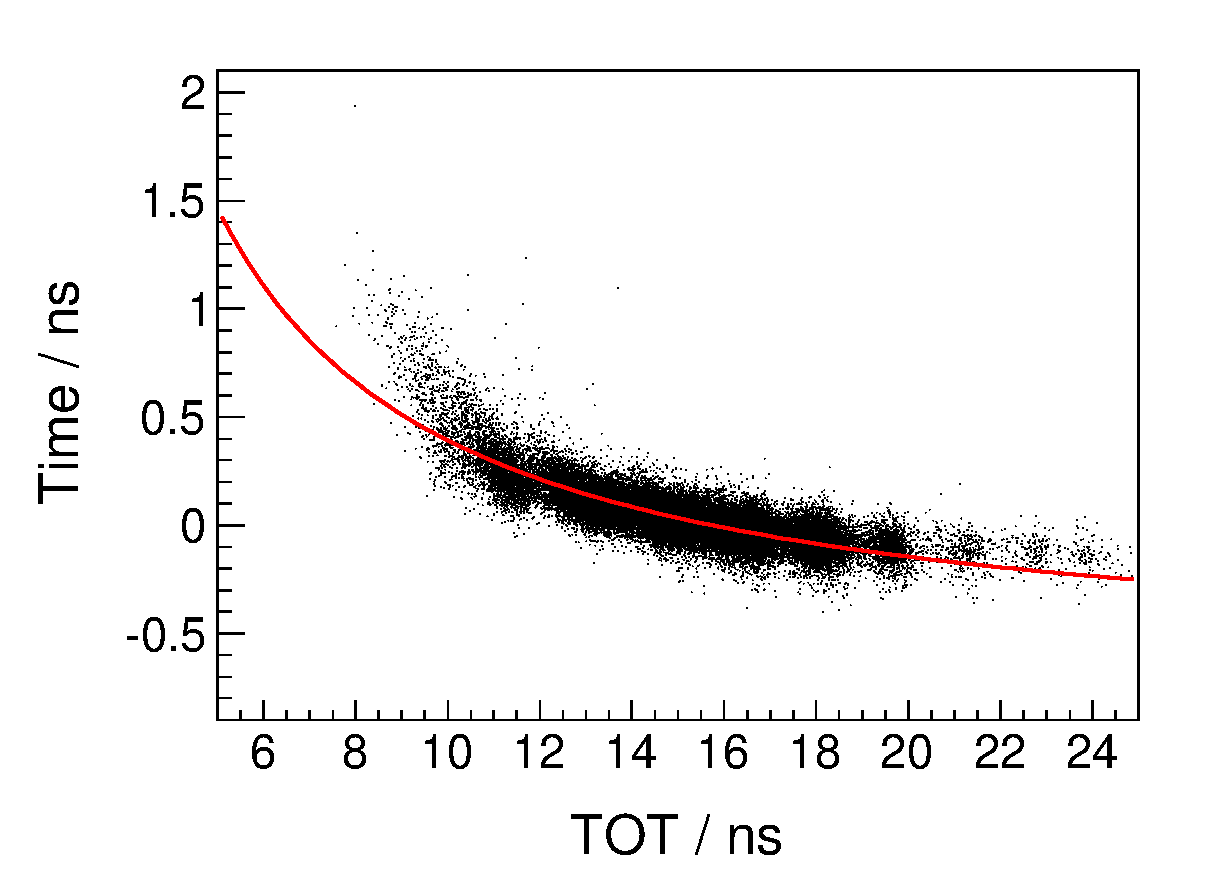
\includegraphics[width=0.9\textwidth]{chap3/1-order.eps}}
  \centerline{(d) 公式~\ref{eq:4}~的拟合}
  \centerline{\label{fig:3-order}}
\end{minipage}
\vfill
\begin{minipage}{0.5\linewidth}
  \centerline{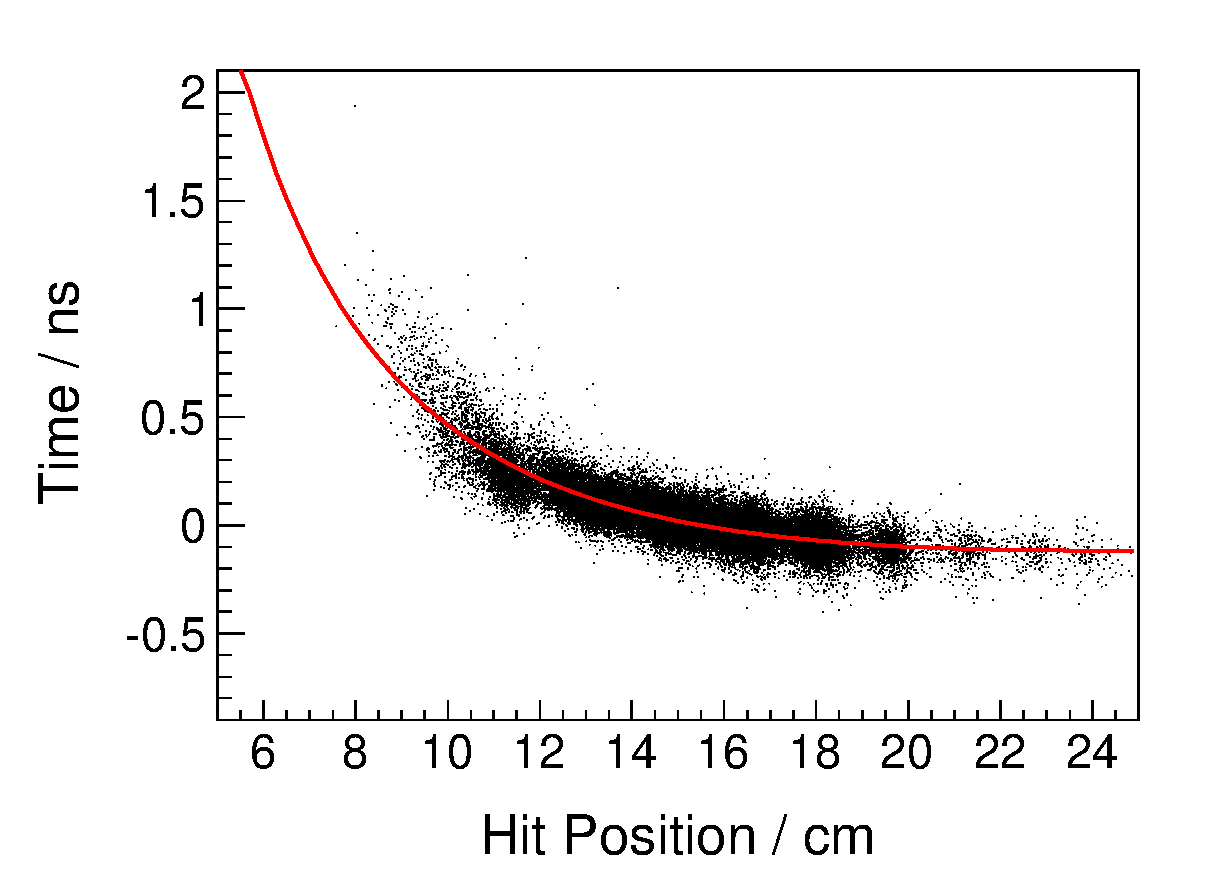
\includegraphics[width=0.9\textwidth]{chap3/ban+1order.eps}}
  \centerline{(e) 公式~\ref{eq:5}~的拟合}
  \centerline{\label{fig:ban+1order}}
\end{minipage}
\hfill
\begin{minipage}{0.5\linewidth}
  \centerline{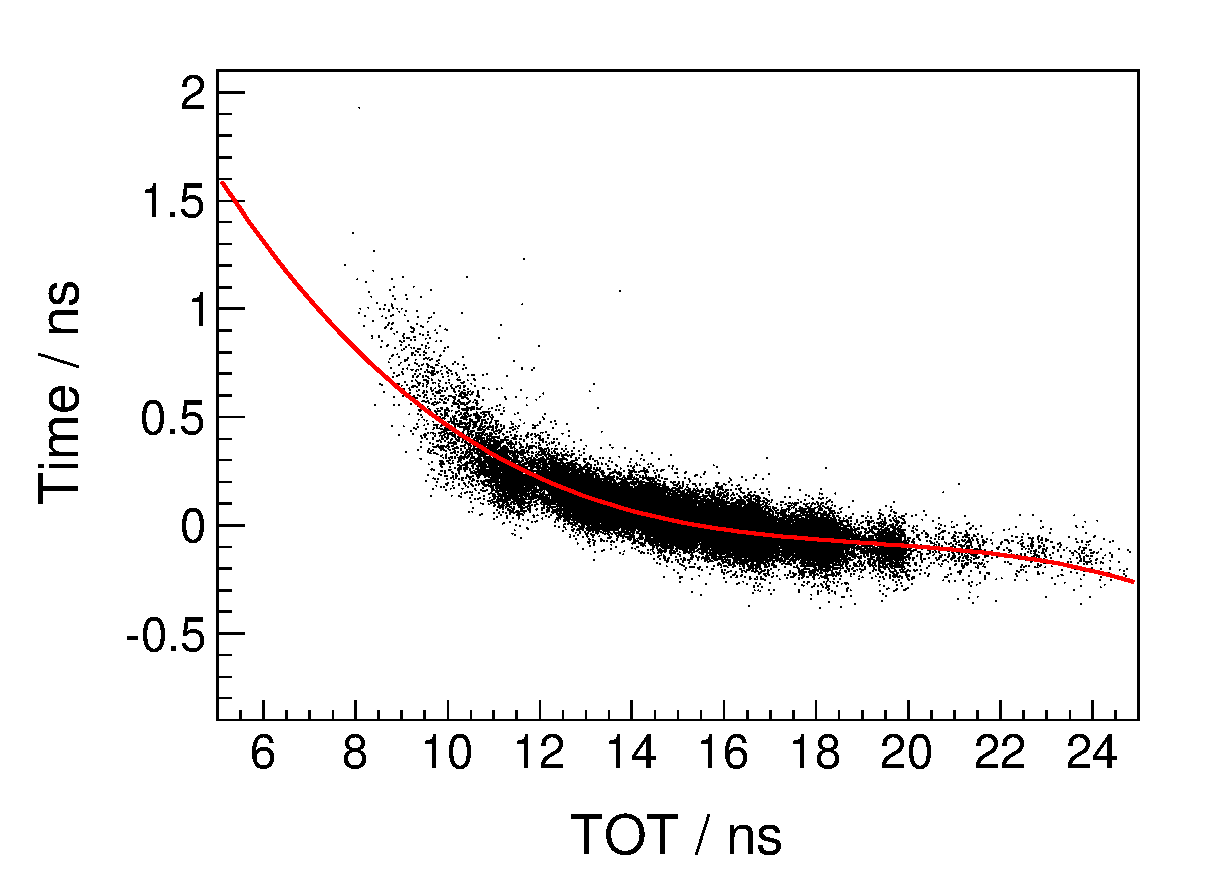
\includegraphics[width=0.9\textwidth]{chap3/pol3-order.eps}}
  \centerline{(f) 公式~\ref{eq:6}~的拟合}
  \centerline{\label{fig:pol3-order}}
\end{minipage}
\caption{几种公式对~TOT~的拟合}
\label{fig:res}
\end{figure}

\begin{table}[h]
    \centering
    \caption{\label{tbl:resolution} 上述公式修正后最终的时间分辨}
  \footnotesize
    \begin{tabular}{lc}
        \hline
        公式& 时间分辨(ps) \\
        \hline
        ${p_{0}+p_{1}/\sqrt{q}}$ & 0 \\
        ${p_{0}+p_{1}/q}$ & 0 \\
        ${p_{0}+p_{1}/q^{2}}$ & 0 \\
        ${p_{0}+p_{1}/q^{3}}$ & 0 \\
        ${p_{0}+p_{1}/\sqrt{q}+p_{2}/q}$ & 0 \\
        ${p_{0}+p_{1}*q+p_{2}*q^{2}+p_{3}*q^3}$ & 0 \\
        \hline
    \end{tabular}
\end{table}

\begin{comment}
\begin{table}[h]
    \centering
    \caption{\label{tbl:scint-detectors} 一些液闪探测器的属性}
  \footnotesize
    %\begin{tabular}{lp{2cm}p{2cm}p{1cm}p{2cm}p{2cm}}
    \begin{tabular}{lccccc}
        \hline
        探测器名称& 质量, kton  & PMT 数目 & 覆盖率 & p.e./\MeV & 时间 \\
                  & (模块数)    & (直径, cm) \\
        \hline
        KamLAND & 0.41 & 1325 (43) + 554 (51) & 34\% & 460 & 2002- \\
        Borexino & 0.1 & 2212 (20) & 30\% & 500 & 2007- \\
        SNO+ & 0.78 & 9438 (20) & 54\% & 400-900 & 2014- \\
        CHOOZ & 0.005 (Gd) & 192 (20) & 15\% & 130 & 1997-1998 \\
        Double Chooz & 0.017 (Gd) (2) & 534/module (20) & 13\% & 180 & 2011- \\
        Daya Bay & 0.160 (Gd) (8) & 192/module (20) & 5.6\% & 100 & 2011- \\
        RENO & 0.032 (Gd) (2) & 342/module (20) & 12.6\% & 100 & 2011- \\
        \hline
    \end{tabular}
\end{table}
\end{comment}
\subsection{确定主项公式}

贴图:贴出两块tofid=55,tofid=?
决定选用 公式~${p_{0}+p_{1}/\sqrt{q}+p_{2}/q}$~为刻度~TOT~的公式。

\section{小结}

上章利用插值方法对MRPC的离线数据进行刻度,这章从另一个角度构造公式入手进行刻度。对于~Z~的修正,采用分~bin~,每个~bin~采用一个非对称的公式~Novosibirsk~拟合,最后对~Z~的修正采用一个三阶多项式拟合。而对于~TOT~拟合,经过比较几种公式,包括每个公式拟合的符合程度,以及随机选用两块比较这些公式的时间分辨。最终选用公式~${p_{0}+p_{1}/\sqrt{q}+p_{2}/q}$~作为~TOT~的修正公式。而下一章双端的修正,更说明了公式~${p_{0}+p_{1}/\sqrt{q}+p_{2}/q}$~是这些公式中拟合最好的,并且适用性最好的。









